\documentclass[a4paper,11pt]{article}
\usepackage[margin=1.0in]{geometry}
\usepackage[utf8]{inputenc}
\usepackage{url}
%%%%%%%%%%%%%%%%%
% EXPERIMENTEX
%
% First, the five primary commands are defined.
%
% The ExperimenTeX commands are first interpreted and
% turned into runs such that afterwards the missing
% output plot files are present for the real LaTeX compilation.
% If the interpreting and plotting have not taken place,
% the LaTeX compilation will simply use placeholders.
%
% Second, two secondary commands related to checksums are defined.
%

% Package dependencies
\usepackage{color}
\usepackage{graphics}
\usepackage{graphicx}

%%%%%%%%%%%%%%%%%%%%%%%%%%%%%%%%%%%%%%%%%%%%%%%%%%%%%%%%%%%%
%
% Format:       \expclass{name-sub}{name-super}
%
% Description:  Declare the existence of class [name-sub], which inherits
%               from class [name-super]. This inheritance means it is of the same
%               experiment type, and inherits all its explines.
%
%               In the rendered document, nothing is shown.
%
\newcommand{\expclass}[2]{}

%%%%%%%%%%%%%%%%%%%%%%%%%%%%%%%%%%%%%%%%%%%%%%%%%%%%%%%%%%%%
%
% Format:       \expinstance{name-inst}{name-super}
%
% Description:  Declare the existence of instance [name-inst], which inherits
%               from class [name-super]. This inheritance means it is of the same
%               experiment type, and inherits all its explines.
%
%               In the rendered document, nothing is shown.
%
\newcommand{\expinstance}[2]{}

%%%%%%%%%%%%%%%%%%%%%%%%%%%%%%%%%%%%%%%%%%%%%%%%%%%%%%%%%%%%
%
% Format:       \expline{name}{expline}
%
% Description:  Add [expline] to the list of explines of instance/class [name].
%
%               In the rendered document, it simply shows [expline] like any other text.
%
\newcommand{\expline}[3][]{{#3}}

%%%%%%%%%%%%%%%%%%%%%%%%%%%%%%%%%%%%%%%%%%%%%%%%%%%%%%%%%%%%
%
% Format:       \expincludegraphics[ic-options]{exp-name}{output-file.ext}
%
% Description:  Add output.ext to the list of expinclude filenames of instance [name-inst].
%
%               In the rendered document, it behaves like \includegraphics.
%               If the output file does not exist (yet), a placeholder image is depicted.
%
\newcommand{\expincludegraphics}[3][]{%
\IfFileExists{../temp/plots/#2/#3}{%
\includegraphics[#1]{../temp/plots/#2/#3}%
}{%
\includegraphics[#1]{example-image-a}%
}%
}

%%%%%%%%%%%%%%%%%%%%%%%%%%%%%%%%%%%%%%%%%%%%%%%%%%%%%%%%%%%%
%
% Format:       \expincludetext{exp-name}{output-file.ext}
%
% Description:  Add output.ext to the list of expinclude filenames of instance [name-inst].
%
%               In the rendered document, it behaves like \input.
%               If the output file does not exist (yet), a placeholder red [X] is put.
%
\newcommand{\expincludetext}[2]{\IfFileExists{../temp/plots/#1/#2}{\input{../temp/plots/#1/#2}\unskip}{\textbf{\textcolor{red}{[\texttt{X}]}}}}

%%%%%%%%%%%%%%%%%%%%%%%%%%%%%%%%%%%%%%%%%%%%%%%%%%%%%%%%%%%%
%
% Format:       \expcodecksum{}
%
% Description:  Code checksum (git commit hash or archive SHA-256)
%               It is imported from file code-checksum.txt
%
\newcommand{\expcodechecksum}[0]{\IfFileExists{code-checksum.txt}{\input{code-checksum.txt}\unskip}{\textbf{\textcolor{red}{[\texttt{not found: code-checksum.txt}]}}}}


% Footnote without marker
\newcommand\markerlessfootnote[1]{%
	\begingroup%
	\renewcommand\thefootnote{}\footnote{#1}%
	\addtocounter{footnote}{-1}%
	\endgroup%
}
\author{}
\title{CodeBind}
\date{}

\begin{document}

\maketitle

\noindent\markerlessfootnote{%
\hspace{-0.58cm}This paper is written using CodeBind.\\%
\url{https://github.com/snkas/codebind-template}\\%
Code checksum: \expcodechecksum{}%
}%
In this document we demonstrate how CodeBind is used. The max-min fairness algorithm implemented is based on section II.B of \cite{nace2006}.

\section{Max-min fairness example}

Under max-min fairness, the addition of flows to the network can \emph{increase} the throughput of some flows.

\expclass{abc}{mmfa}
To demonstrate this, we use a simple topology of three nodes with two directed edges:
\expline{abc}{the edge from A to B has a capacity of 1 unit},
and the \expline{abc}{the edge from B to C has a capacity of 1 unit}.

\expinstance{abc-one}{abc}
In the first experiment, we start the following flows: \expline{abc-one}{one from A to B} (path is A$\rightarrow$B), \expline{abc-one}{one from B to C} (path is B$\rightarrow$C), and \expline{abc-one}{one from A to C} (path is A$\rightarrow$B$\rightarrow$C).
This results in a max-min fair allocation of \expincludetext{abc-one}{flow-allocation-A-B.txt}, \expincludetext{abc-one}{flow-allocation-B-C.txt} and \expincludetext{abc-one}{flow-allocation-A-C.txt} for each type respectively.

\begin{center}
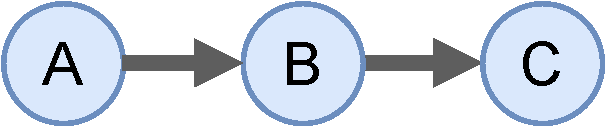
\includegraphics[width=4.5cm]{figures/topology-example.pdf}
\end{center}

\expinstance{abc-vary}{abc}
However, suppose that one would increase the number of flows from A to B. What would happen to the flow from B to C? In the second experiment, as before we start \expline{abc-vary}{one flow from B to C} and \expline{abc-vary}{one flow from A to C}. \expline{abc-vary}{We vary the number of flows from A to B between 1 and 4}. The addition of extra flows from A to B results in the flow from A to C being bottlenecked there, resulting in the flow from B to C being allocated more.

\begin{center}
\expincludegraphics[width=8cm]{abc-vary}
{num-flows-A-B-vs-flow-allocation-B-C.pdf}
\end{center}


\bibliographystyle{plain}
\bibliography{bibliography}

\end{document}
